\subsection{Número de coordinación}

De la misma manera que se utilizaron las distribuciones radiales parciales, se pueden
obtener los números de coordinación para un dado tipo de átomo utilizando la ecuación
\ref{eq:cn} definida en la sección \ref{ss:cn} con la $g(r)$ correspondiente. Debido
a que en los materiales amorfos la primera y la segunda esfera de coordinación pueden 
llegar a estar superpuestas, el límite superior de integración no está definido 
unívocamente para todas las concentraciones consideradas \cite{lamparter1995}.
El número de coordinación promedio para átomos de Si vecinos de otros átomos 
de Si se calculó utilizando un radio de 
corte de 3 \AA. Lo mismo se realizó para Li-Li definiendo un radio de corte de 
4 \AA. Para el caso de Si-Li se utilizó el criterio de considerar como radio de 
corte el valor $r$ para el cual la $g(r)$ presenta un mínimo entre los dos picos
a primeros y segundo vecinos. Los resultados se muestran en la Figura 
\ref{fig:cn}a.
\begin{figure}[h!]
    \centering
    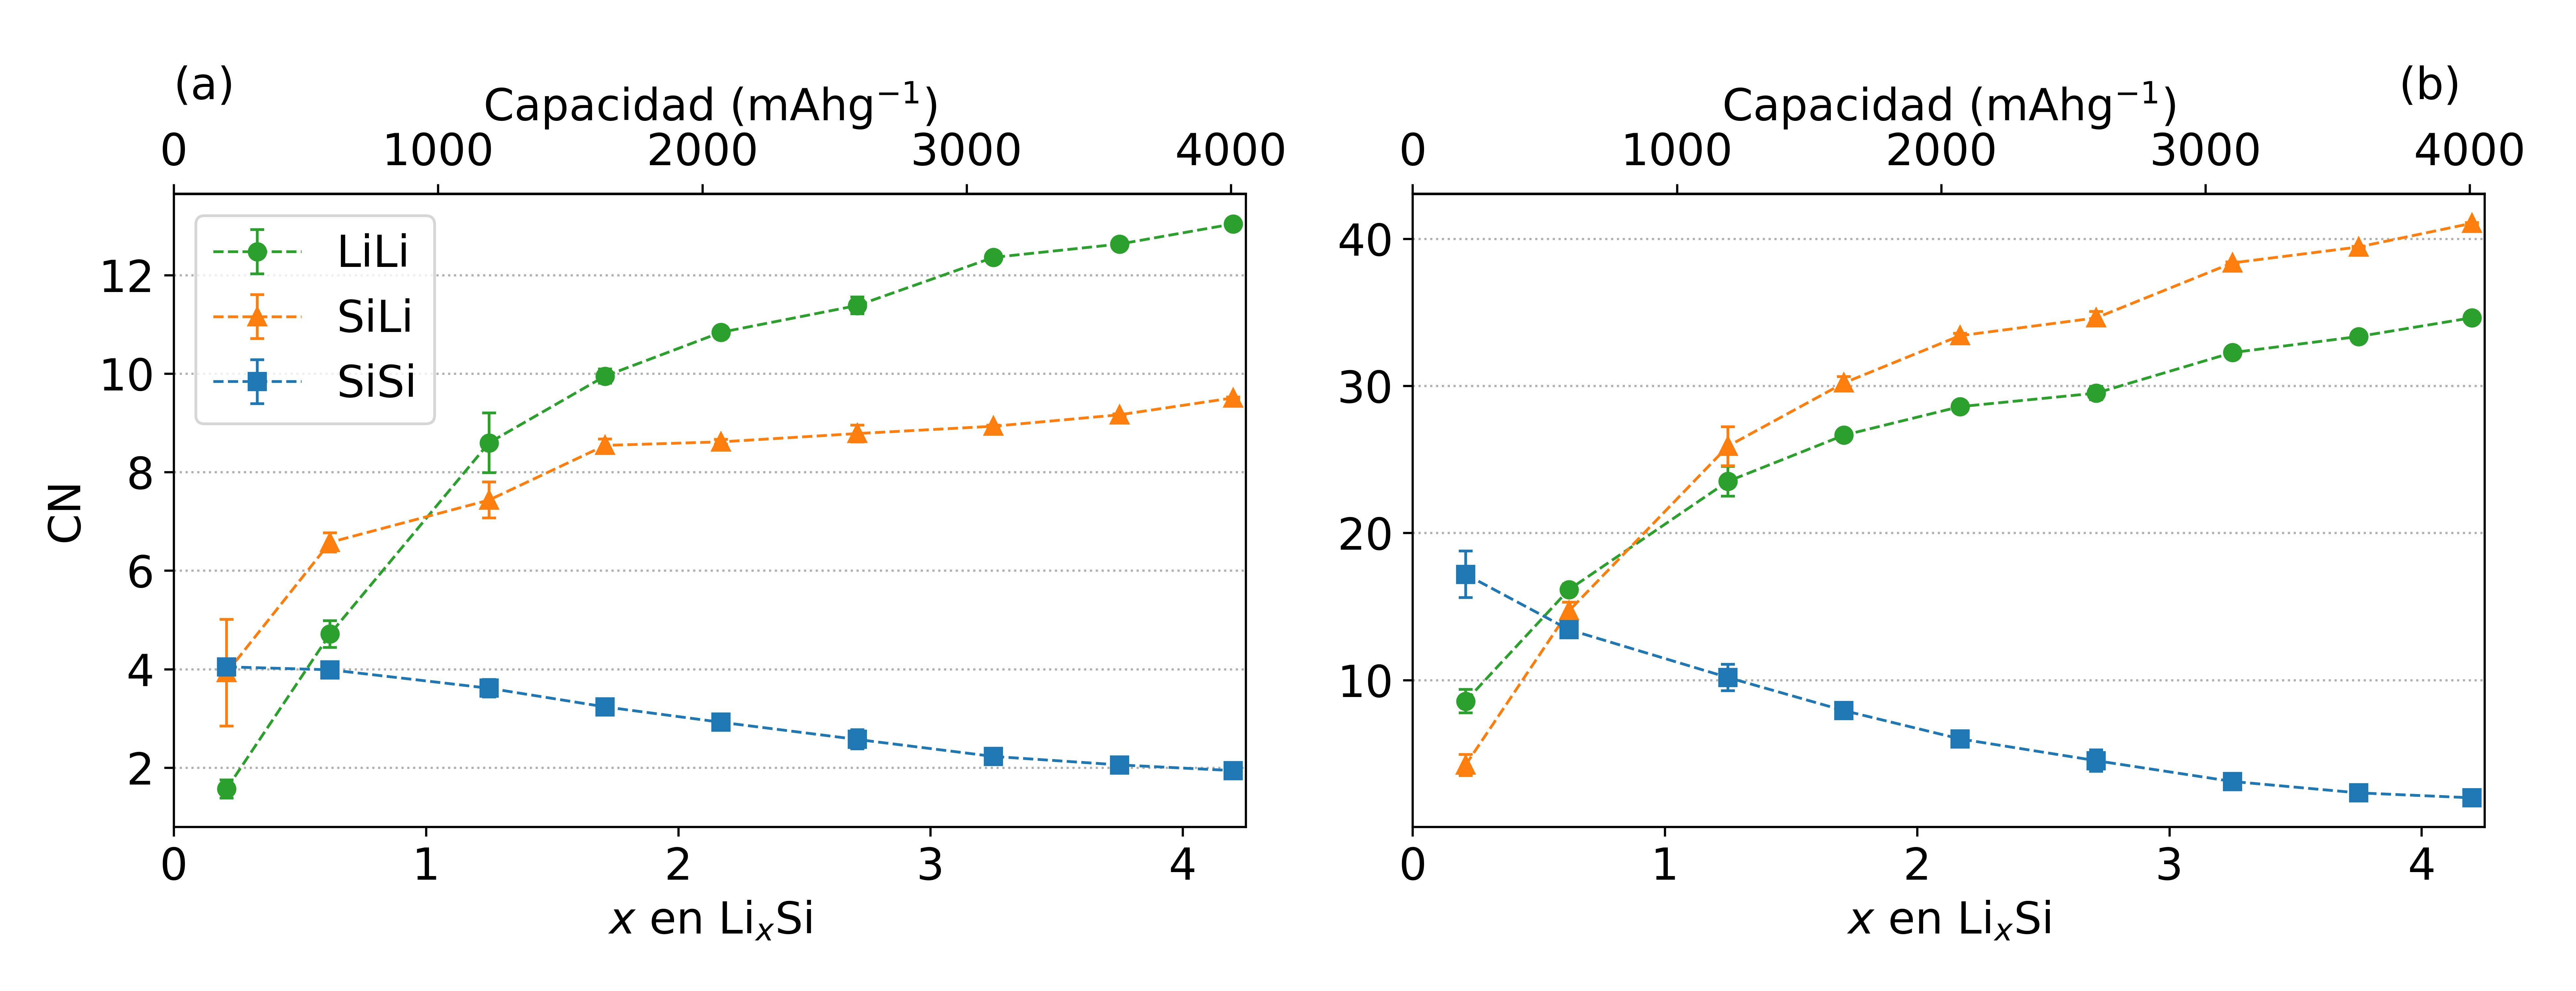
\includegraphics[width=\textwidth]{Silicio/caracterizacion/resultados/cn/cn.png}
    \caption{Número de coordinación en función de la concentración de litio para
    Li-Li, Si-Si y Si-Li. Como radios de corte se utilizaron las distancias 
    del pico de la RDF correspondiente. En los casos en que no se aprecia la barra
    de error, la misma es menor que el tamaño de los puntos. (a) Primero número 
    de coordinación. (b) Segundo número de coordinación.}
    \label{fig:cn}
\end{figure}

Para el caso del CN$_{\text{Si}-\text{Si}}$, se tiene que esta cantidad decrece de 4 a 2, a 
medida que la concentración de Li aumenta. Esto indica que a valores pequeños de 
$x$ la estructura de Si mantiene sus conexiones tetraédricas, mientras que para
valores grandes de $x$ el Si tiende a formar cadenas periódicas unidimensionales.
En la red de silicio amorfa, analizada con más detalle en la sección 
\ref{s:clusters}, se presenta una estructura 3d-periódica para valores bajos de 
$x$, donde el CN se encuentra alrededor de 4. Luego, se alcanza una estructura 1d-periódica 
para valores grandes de $x$, donde los enlaces Si-Si tienden a formar 
cadenas, que pueden verse para $x = 3.75$ donde se tiene CN = 2.05, por ejemplo.
El CN de Si-Li y Li-Li presenta valores pequeños para concentraciones 
bajas y aumenta monótonamente hasta alcanzar valores de 10 y 12, respectivamente, 
que se asemejan al valor de una estructura de empaquetamiento compacto.

Los resultados para el segundo número de coordinación se presentan en la Figura 
\ref{fig:cn}b. Estos resultados se obtuvieron considerando un cascarón con un 
radio de corte interno y otro externo, elegidos de manera tal que incluyan el 
segundo pico de la RDF. La elección de dichos valores varió dependiendo del tipo
de átomos que se consideraron. En todos ellos se tomó como radio de corte interno 
el radio de corte del primero número de coordinación. Luego, para el radio de 
corte externo se utilizaron valores de 5.0 \AA\ para Si-Si y 6.0 \AA\ para Li-Li
y Si-Li.

Para los valores de CN$_{\text{Si}-\text{Si}}$ se observa un aumento para concentraciones bajas
de Li, si se lo compara con el CN de primeros vecinos. Para valores mayores de $x$,
se puede ver cómo el valor de CN también tiende a 2, lo cual es coherente con la
formación de cadenas que se notó previamente. La tendencia cualitativa del segundo
CN para Li-Li y Si-Li es la misma que la observada en el primer CN, sólo que ahora
empieza en un valor cercano a 5 y tiende a 35 y 40, respectivamente. Este valor 
es mucho mayor que el que se tiene para los segundos vecinos en una estructura 
de empaquetamiento compacto, que es 6 para la estructura cristalina FCC. Incluso 
es mayor a la suma del segundo (6) y del tercer vecino (24) esperado para la red 
FCC.
